\appendix

\section{Cross validation of the ML algorithms}  \label{app:crossval}

To obtain the optimal hyperparameters of our \ac{ML} algorithms, we perform a cross validation across different values of the algorihtms' parameters. We apply the algorithms on our O2 dataset for different choices of parameters, and we select the combination that gives the highest accuracy. 

\subsection{K-Nearest Neighbors}

Regarding the \ac{KNN} algorithm, $k$-fold cross validation implemented in scikit-learn~\cite{Pedregosa:2011ork} was used, with $k = 10$ folds, . as this choice is commonly used in applied machine learning. As consistency checks, we also applied different numbers of folds ($k = 4$ and $k=5$) and obtained consistent results for all the cases.  The dataset employed to cross validate is $D=D_R\oplus D_S$. 

The characteristic hyperparameters of the \ac{KNN} algorithm are the number of neighbors ($K$), the metric used distance computation, the algorithm to obtain the nearest neigbors, and the weight function for prediction. In table~\ref{tab:KNN_crossval_tab} we depict several combinations of these parameters and the resulting accuracy after cross validating. One can note that the accuracy is practically insensitive to the choice of hyperparameters.


\begin{table}[h]
\begin{tabular}{c|c|c|c|c}
\hline
Neighbors   & Metric & Weights & Algorithm & \multicolumn{1}{|c}{Accuracy} \\ \hline
2                                   & Manhattan                   & Distance                    & BallTree                   &  0.9399                                  \\
2                                   & Euclidean                   & Distance                    & KDTree                   & 0.9392                           \\
2                                   & Manhattan                   & Uniform                    & Auto             &                    0.9359  \\
8                                   & Manhattan                  & Distance                   & BallTree &                    0.9485 \\
8                                   & Euclidean                 & Distance                   & KDTree             &                       0.9477 \\               
8                                   & Manhattan                   & Uniform                   & Auto              &                          0.9468 \\
20                                   & Manhattan                   & Distance                   & BallTree &                  0.9469 \\
20                                   & Euclidean                   & Distance                   & KDTree              &                       0.9459 \\               
20                                   & Manhattan                   & Uniform                   & Auto              &                          0.9437 \\
\hline
\end{tabular}
\caption{Values of the accuracy for different combinations of the hyperparameters. The accuracy in all cases is larger than $0.935$.}
\label{tab:KNN_crossval_tab}
\end{table}

In Figure~\ref{fig:crossvalKNN} we show the dependence of the accuracy on different choices of hyperparameters, keeping fixed the algorithm used to compute the nearest neighbors, which is the BallTree.

\begin{figure*}%[h]
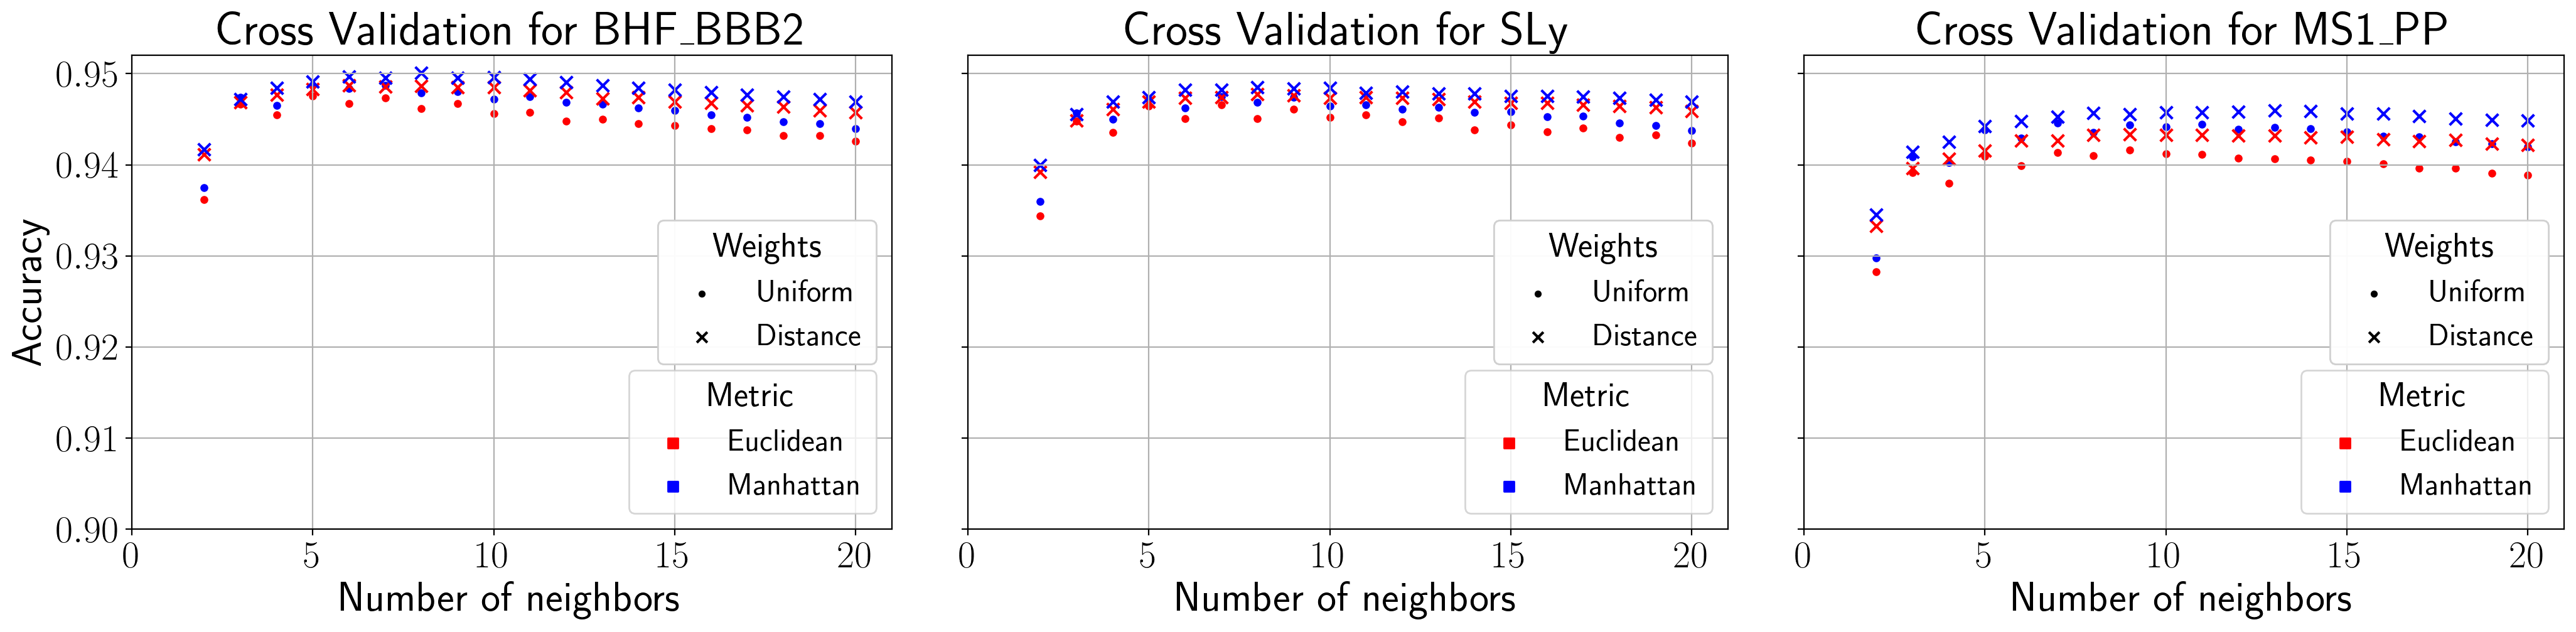
\includegraphics[width=\linewidth]{cross_val_KNN}
\caption{Dependence of the accuracy of the KNN algorithm with the number of neighbors. The red (blue) color corresponds to the Euclidean (Manhattan) metric and the dots (crosses), to uniform (distance) weights.  The algorithm to compute the closest neighbors is fixed to the BallTree. algorithm.  There is not a strong dependence with the number of neighbors when considering more than 5 neighbors. }
\label{fig:crossvalKNN}
\end{figure*}

We found that the optimal hyperparameters were the same for all the equations of state, except of the number of neighbors, which changed between 6 and 12. We margilanize over all the equations of state using the Bayes' factors presented in~\cite{Ghosh:2021eqv}. The marginalised optimal number of neighbors turns out to be 8. However, as one can see in Fig.~\ref{fig:crossvalKNN}, there is not a considerable change in accuracy when a larger number of neighbors is used. The fixed hyperparameters used for our KNN implementation are shown in Table~\ref{tab:KNN_opt_params}.


\begin{table}[h]
\begin{tabular}{c|c|c|c}
\hline
Nº of neighbors   & Metric & Weights & Algorithm  \\ \hline
8  & Manhattan  & Distance & BallTree \\ 
\hline
\end{tabular}
\caption{Table with the optimal hyperparameters for the KNN algorithm. These values are the ones with which we train and test the algorithm, and build the Bayesian probabilities.} \label{tab:KNN_opt_params}
\end{table}


\subsection{Random Forest}

In order to apply the crossvalidation to the Random Forest algorithm, we use the training ($D_R$) and testing ($D_S$) data sets presented in Section~\ref{probability}. We select possible values for the different hyperparameters and compare the accuracies of the resulting forests. Differently from KNN, in RF we do not use the $k$-fold crossvalidation technique. This is because the implementation of RF we use admits the bootstrap technique in the training: each tree in the forest access a random subset of the training data, therefore achieving the same effect.

The hyperparameters studied are the number of trees in the forest, the method to compute the information gain after each node split (the options are gini or entropy),the maximum number of features that are considered in each node (we use the square root of the total number of features, or all of them) and the maximum depth that the trees can reach. For the depth of the trees we consider two different options: None, which consists in letting the trees grow until isolating data points at the leaves, and 15. We choose this number because it is half of the average depth obtained with the None option.

Taking the configuration leading to the highest score for every EOS we marginalize the best options using the Bayes factors. We obtain that for all EoS we should use 81.017 trees, "entropy" criterium, the square root of the number of features at split and depth equal to 15.

\begin{table}[h]
\begin{tabular}{|l|c|}
\hline
Trees& 81.02 \\
Criteria (0-gini, 1-entropy)& 0.9577 \\
Features (0-sqrt, 1-All)& 0.3902  \\
Depth (0-15 depth, 1-Let grow)& 0.0000 \\ \hline
\end{tabular}
\caption{Table with the optimal hyperparameters for the RF algorithm. \label{tab:RF_cross_params}}
\end{table}

In table \ref{tab:RF_cross_params} we present the results of the marginalization of the hyperparameters over the EOS. Notice that for all EOS and independently of the values of the other hyperparameters, we always obtain a higher accuracy with depth equal to 15. The "entropy" criterium is chosen for almost all EOS, while the decision of the quantity of features to consider is more tight.

In Figure~\ref{fig:crossvalRF} we plot the scores obtained during crossvalidation, fixing the depth equal to 15. The difference in the accuracy between different configurations is very small and therefore we decided to reduce the final number of trees to 50. The idea to make this algorithm run in low-latency favors smaller files that can be loaded fast. Giving the difference in accuracy and in size of the trained model, we restrict ourselves to 50 trees.

\begin{figure*}%[h]
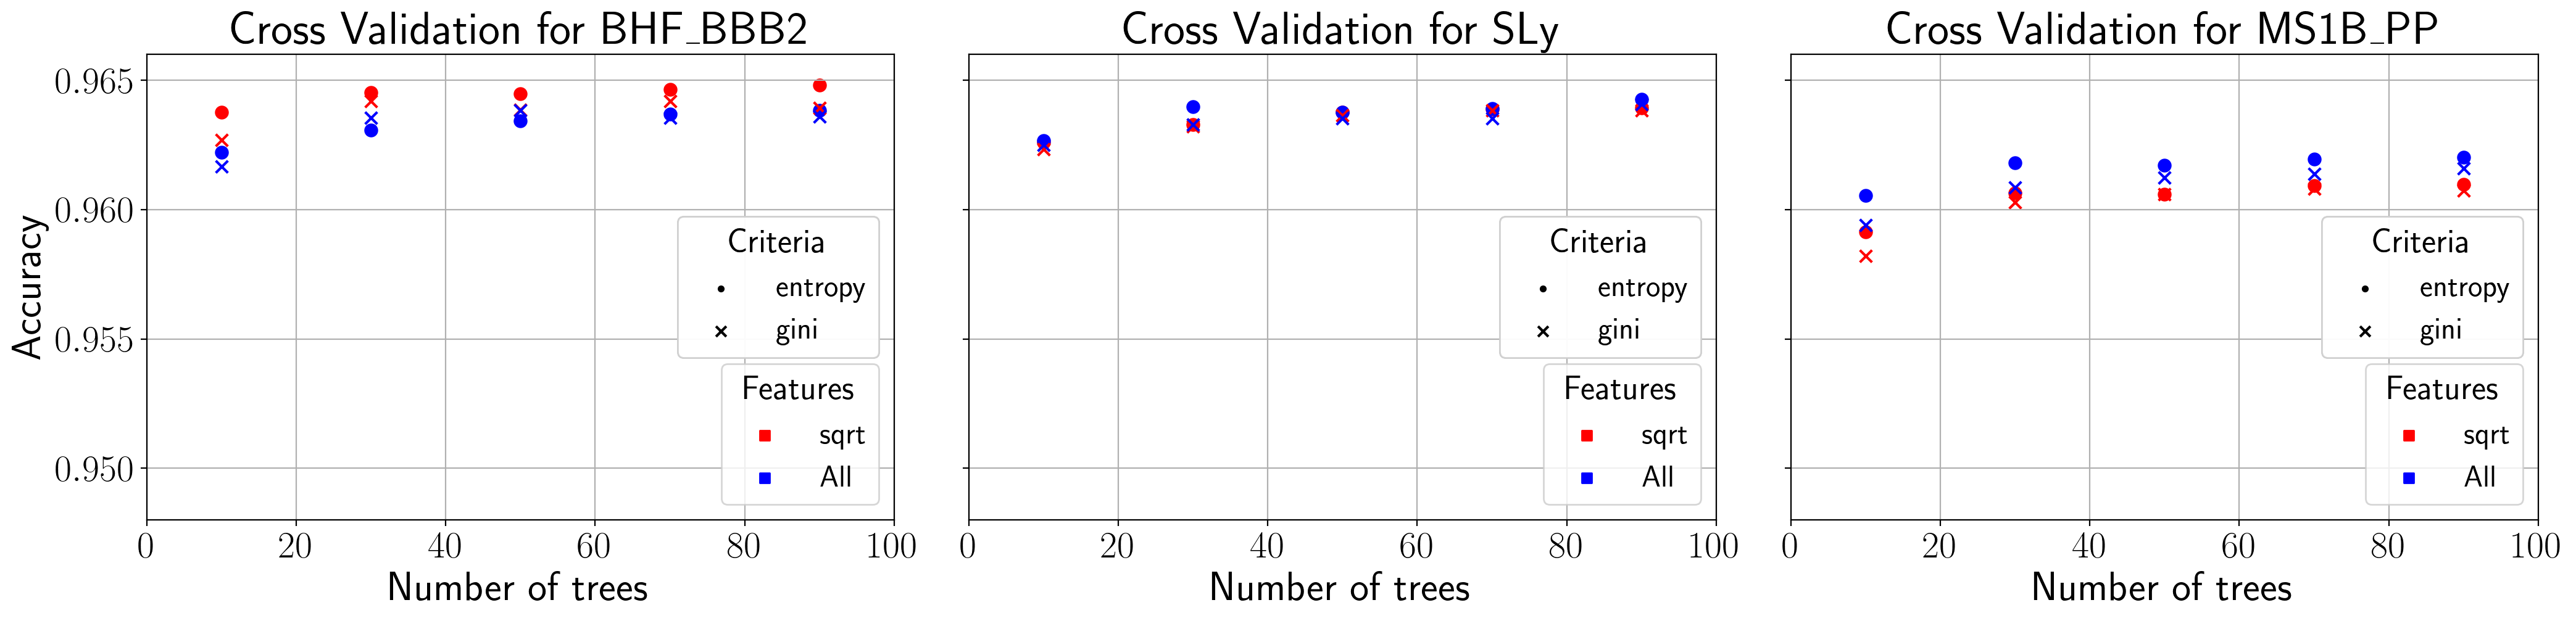
\includegraphics[width=\linewidth]{cross_val_RF}
\caption{Dependence of the accuracy of the RF algorithm with the number of trees. The red (blue) color corresponds to "sqrt" ("all") features and the dots (crosses), to "entropy" ("gini") criteria.  The depth of the trees is fixed to 15.  The accuracy lays between 0.960 and 0.965 in all cases.}
\label{fig:crossvalRF}
\end{figure*}

\section{Comparison between our algorithms and the current LVK implementation}  \label{app:comparison}

To make a comparison between the current \ac{KNN} implementation~\cite{Chatterjee:2019avs} with our multi-label \ac{KNN} and \ac{RF} schemes, we depict in Figure~\ref{fig:rocO2_all} the ROC curves for the three algorithms. For fair comparison,  we trained the LVK's \ac{KNN} classifier for two cases (\hasns and \hasrem) independently., resulting in a binary label approach.  In this case, we use the hyperparameters currently set in the low-latency implementation: $K = 2n + 1 = 11$ neighbors, (where $n$ is the number of features), the Mahalanobis metric and the neighbors are weighted by the inverse of their distance.  These two classifiers were trained in the same 70$\%$ of the O2 dataset\footnote{In the current LVK implementation, the algorithm is trained on the entirety of the dataset $D$, which leaves us without enough testing. Here, we chose a 70$\%$-30$\%$ split and hence made a comparison accordingly. } (the $D_R$ subset) as our multi-label approaches. The ROC curve below is made on the remaining 30$\%$ of the dataset (the $D_S$ subset). As expected,  the multi-label RF approach has a high TPR across the range of FPR for both \hasns and \hasrem . Both multi-label KNN and binary label KNN perform similarly for both scenarios.Please note that these ROC curves comparison is done in the same was as in Figures~\ref{fig:rocO2_KNN} and~\ref{fig:rocO2_RF}, before defining Bayesian probabilities since they are constructed from the testing set. 

\begin{figure*}%[h]
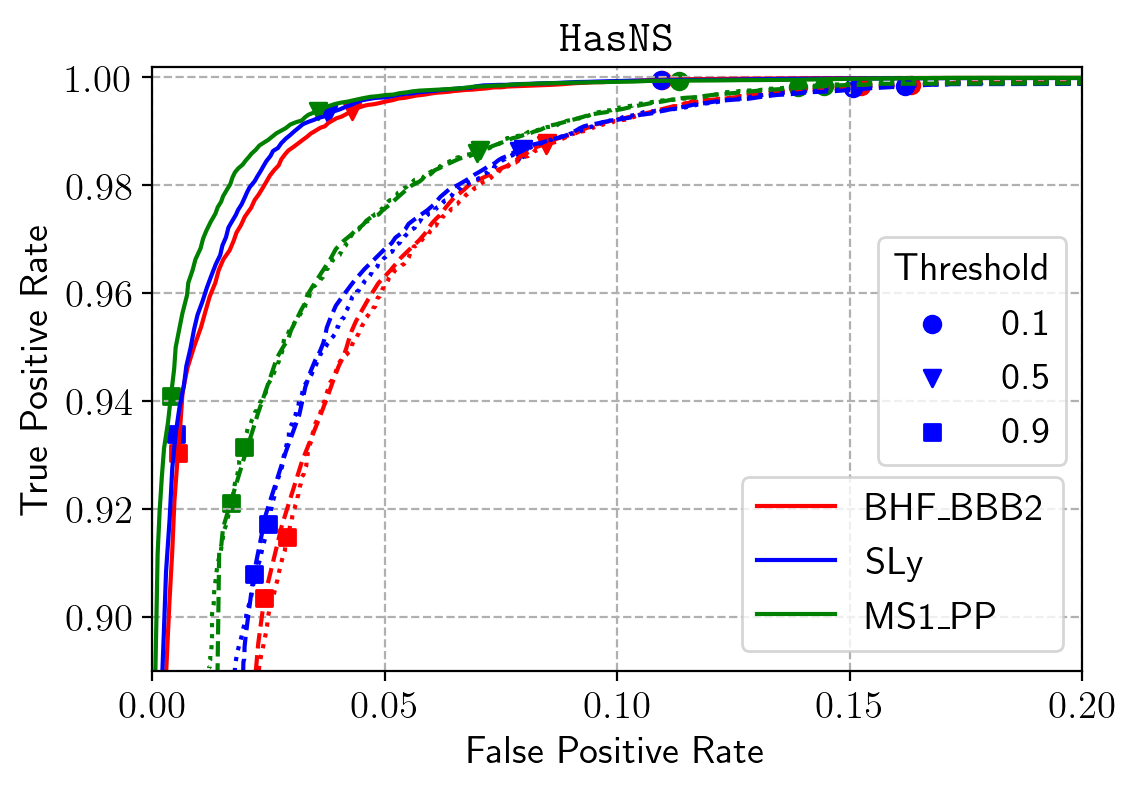
\includegraphics[width=0.47\linewidth]{ROC_O2testing_all_impl-NS}
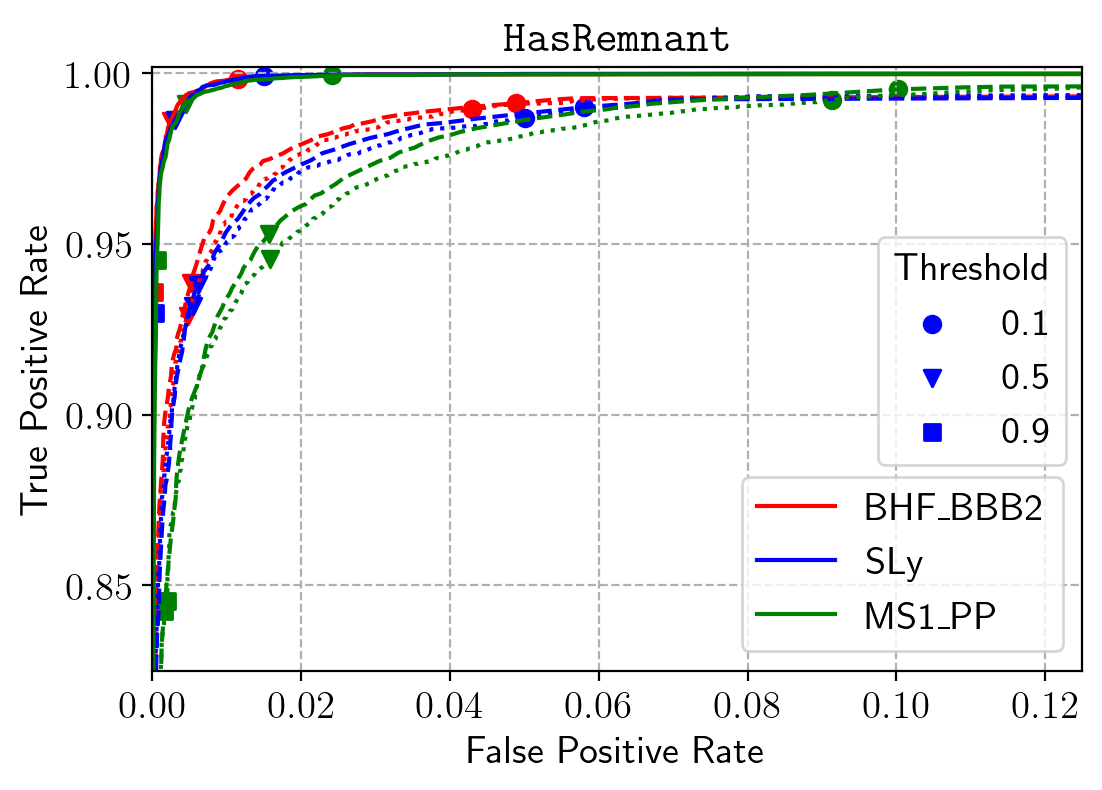
\includegraphics[width=0.45\linewidth]{ROC_O2testing_all_impl-REM}
\caption{.}
\label{fig:rocO2_all}
\end{figure*}




